\chapter[Estimating the Cosmic Background Rate with Backward Monte Carlo
Simulation]{Estimating the Cosmic Background Rate \\with Backward Monte Carlo
Simulation}\label{ch:cosmics}

% \begin{markdown}

% 1. Intro to BMC: relation to adjoint MC (find refs), maybe diagram

% 2. Physics: how we use BMC to determine rates of cosmic events: equations for
% flux, sampling PDF, BMC weights, topography map of J-PARC

% 3. Integration into ICEDUST: implementation of sampling methods, event loop, output to
% oaRooTracker format
% + `https://gitlab.in2p3.fr/comet/ICEDUST_packages/-/merge_requests/534`
% + `https://gitlab.in2p3.fr/comet/ICEDUST_packages/-/wikis/Backward-Monte-Carlo-sampling-with-SimBackwardMC#rate-calculation`

% 3. Actual estimation of background rate in Phase-I, maybe just quoting V's
% result

% ---

% \end{markdown}

% Intro
Cosmic ray-induced events represent a significant part of the expected
backgrounds in the COMET experiment, as discussed in
Section~\ref{sec:backgrounds}. Cosmic muons irradiate the Earth at irregular
intervals and have a wide energy spectrum, hence some fraction of them will be
able to mimic the conversion signal by entering the COMET detector system. In
this chapter, we discuss how backward Monte Carlo simulation helps to
efficiently estimate the background rate from cosmic ray-induced events.

\section{Backward Monte Carlo simulation}

Estimating the rate at which cosmic muons might produce signal-like events is
computationally expensive through standard Monte Carlo simulation methods. This
is due to the fact that the source of cosmic muons, i.e.\ the atmosphere, has a
much greater spatial extent than the active detector region. Hence, most cosmic
events generated from an atmospheric source will miss the detector completely
and not contribute in the estimation of the background rate, resulting in wasted
computation time.

A backward (or adjoint) Monte Carlo simulation is one where the flow of particle
transport is reversed, i.e.\ events are generated in the sensitive detector
volume and propagated backward in time until they reach the source. This method
was initially used in 1967 to estimate gamma-ray and neutron radiation doses in
nuclear reactors~\cite{doi:10.13182/NSE68-A19235,doi:10.13182/NSE69-A19116}.
More recently, backward MC has also been integrated into Geant4
simulations~\cite{DESORGHER2010247} for dosimetry in space, reversing the
electromagnetic physics of electrons, protons and ions.

In the case of muons, a backward transport method was developed by Niess et
al.~\cite{Niess_Barnoud_Carloganu_Menedeu_2018} in the context of muon
tomography. It was later adapted to the COMET experiment in order to refine
estimations of the background rate from cosmic rays. 
% This chapter discusses the
% backward MC method for cosmic muons, how it is applied to COMET and the
% resulting rate estimations in COMET Phase-I.

\begin{figure}
    \centering
    \begin{subfigure}[t]{0.49\textwidth}
        \centering
        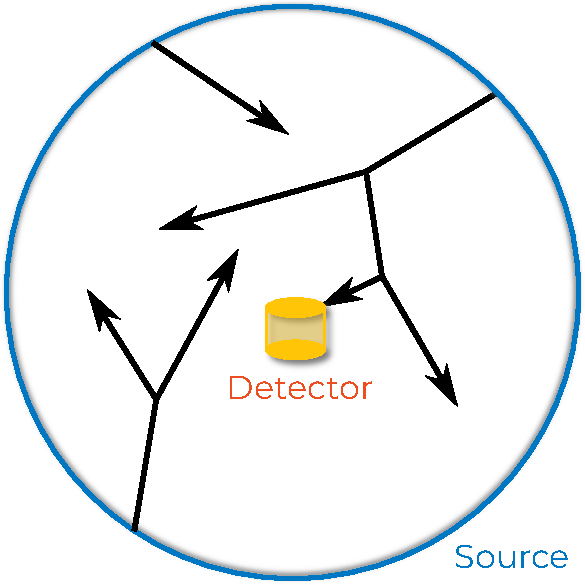
\includegraphics[width=0.75\textwidth]{chapter5/bmc_setup.pdf}
        \caption{Forward MC.}
    \end{subfigure}
    \hfill
    \begin{subfigure}[t]{0.49\textwidth}
        \centering
        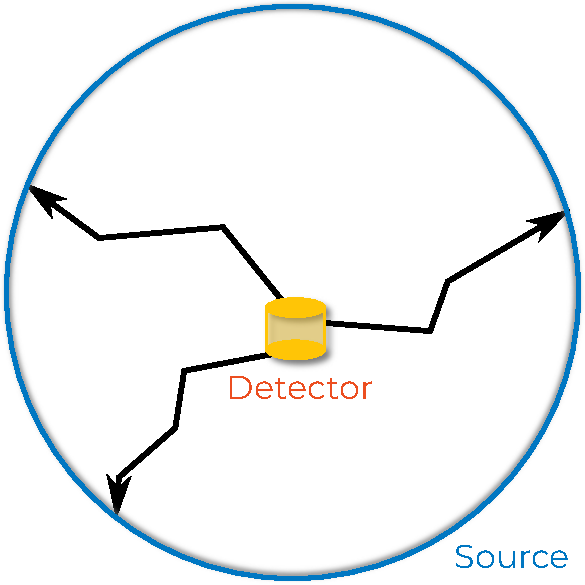
\includegraphics[width=0.75\textwidth]{chapter5/bmc_setup_backward.pdf}
        \caption{Backward MC.}
    \end{subfigure}
    \caption{
        Comparison of the forward and reverse (also called adjoint or backward)
        configurations of Monte Carlo simulation, in the case where a small
        detector volume is surrounded by a comparatively large particle source.
        Reversing the flow of particle transport means that sampled events are
        more likely to contribute toward the rate estimation.
    }
    \label{fig:bmc_configuration}
\end{figure}

%\subsection{Method}
In standard Monte Carlo simulations, events are generated by a source and
propagated forward in time according to their equations of motion and
interaction cross-sections within any surrounding medium. In a situation where
the source is large compared to the sensitive detector volume, as illustrated in
Figure~\ref{fig:bmc_configuration}, events have a high probability to miss the
detector and contribute nothing toward the result.

In backward MC, events are generated according to an arbitrary probability
density function (PDF) around the detector volume. The overall sampling PDF is
typically the composite of a position, direction and energy sampling
distributions, i.e.\ 
\begin{align}\label{eq:sampling_pdf}
p(\bm{x}, \bm{p}, E) = p(\bm{x}) \ \times\  p(\bm{p}) \ \times\  p(E),
\end{align}
where $p$ denotes an arbitrary PDF whose integral is 1, $\bm{x}$ denotes
position, $\bm{p}$ direction and $E$ energy. If more than one particle type is
considered, the discrete distribution of particles can also enter
Equation~\ref{eq:sampling_pdf}. In our case, both cosmic muons and anti-muons
are relevant, and they are sampled identically in equal proportions.

\sepfootnotecontent{A}{Reference~\cite{DESORGHER2010247} also provides a more
thorough discussion of adjoint cross-sections, weights, weight corrections and
source normalisation.}

Each event $i$ is propagated backward using adjoint transport and interaction
kernels such that the particle undergoes reverse energy loss and various
discrete processes, while moving backward toward the source. At each step $j$ of
the propagation, a multiplicative weight $w^i_j$ is computed given the path
taken and the interactions along it. When the particle reaches the source, the
directional flux at the source $\phi_\mathrm{s}$ is used as a normalisation
factor to yield a weighted event flux
$$
\phi(\bm{x}'_i, \bm{p}'_i, E'_i) = \prod_j w^i_j\ \times\ 
\phi_\mathrm{s}(\bm{x}'_i, \bm{p}'_i, E'_i),
$$
where $\bm{x}'$, $\bm{p}'$ and $E'$ denote respectively the position, direction
and energy of the particle upon reaching the source.

The weighted event flux $\phi$ is related to the event rate $R$ by the
inverse of the sampling PDF of Equation~\ref{eq:sampling_pdf} used to generate
the event initially:
\begin{align*}
R\,(\bm{x}_i, \bm{p}_i, E_i, \bm{x}'_i, \bm{p}'_i, E'_i) = 
    \frac{\phi_i(\bm{x}'_i, \bm{p}'_i, E'_i)}{p(\bm{x}_i, \bm{p}_i, E_i)}.
\end{align*}
Since the rate depends on the position, direction and energy of the particle at
the source, it is susceptible to variation across backward runs because of the
stochastic aspect of Monte Carlo transport. Hence, backward transport is
repeated $N$ times for each event to find the average rate
\begin{align}\label{eq:avg_rate}
\overline{R}\:(\bm{x}_i, \bm{p}_i, E_i)
    &= \sum_{k=1}^N R\,(\bm{x}_i, \bm{p}_i, E_i, \bm{x}'_k, \bm{p}'_k, E'_k) \nonumber\\
    &= \frac{1}{p(\bm{x}_i, \bm{p}_i, E_i)} \ \times\ \frac{1}{N} \sum_{k=1}^N \phi(\bm{x}'_k, \bm{p}'_k, E'_k),
\end{align}
smearing out the dependence on $\bm{x}'$, $\bm{p}'$ and $E'$. Given a large
enough $N$, i.e.\ a significant enough sample of backward transports, the sum of
weighted fluxes becomes equivalent to an integration over the possible transport paths
and interactions, and Reference~\cite{DESORGHER2010247} demonstrates that the
obtained results are consistent with forward Monte Carlo\sepfootnote{A}.



% Desorgher on the matching between forward and backward MC:
%  The Monte Carlo sampling of a big enough number of reverse tracks is
%  equivalent to the integration of the weight W over all independent variable
%  (E1,O1,Sd,x1,E0, ...) summed over all type of reverse reactions, atomic
%  elements, adjoint primaries, and adjoint secondaries. In this integration the
%  cases where more than one reaction and no reaction occur are also considered
%  and only the tracks reaching the external source are accounted for. By this
%  way the same answer is obtained as in the forward case.





\section{Application to COMET Phase-I}
% Here, talk about the COMET setup: 
% + We want to estimate the rate of background events caused by 
%   muons+secondaries hitting the detector
% + Thus, we sample muons+/- around the envelope of the CRV, according to [spell
%   out PDF]
% + We apply backward MC up to an atmospheric muon flux model at altitude X,
%   tabulated from CORSIKA etc.
% + We can first estimate the cosmic muon rate on each surface of the CRV
%   Show plots etc.
% + From the events generated at the CRV envelope, it is also possible to
%   propagate forward to determine which events might produce signal-like
%   tracks.
% + Once this is done, we use the results from backward propagation to estimate
%   rate of background-inducing cosmic muons, qed.
In the COMET Phase-I experiment, the cosmic ray veto (CRV) described in
Section~\ref{sec:crv} will enclose the Cylindrical Detector in order to help
identify events caused by cosmic muons. Backward Monte Carlo simulation can be
used to estimate how many background events originating from cosmic rays will
occur over the experiment's run time. 

\subsection{Event sampling}
In the context of Phase-I, we define a sampling envelope around the CRV, where
muons and anti-muons will be generated and backward-propagated. Muons and
anti-muons are sampled uniformly over this envelope, a box which is decomposed
into six planes. The direction is distributed according to Lambert's cosine law,
i.e.\ 
$$
p(\bm{p}) = 
    \frac{1}{N_{\bm{p}}} \ \hat{\bm{p}} \cdot \hat{\bm{n}} = 
    \frac{1}{N_{\bm{p}}}\:\cos(\theta),
$$
where $\theta$ is the angle between $\bm{p}$ and the normal to the plane
$\hat{\bm{n}}$. $N_{\bm{p}}$ is the normalisation term satisfying 
$\int p(\bm{p}) \: \textnormal{d}\bm{p} = 1$.
The energy distribution is an inverse law, i.e.\ 
$$
p(E) = \frac{1}{N_E}  \frac{1}{E},
$$
where $N_E$ is the normalisation factor. 
This sampling PDF allows us to generate muons and anti-muons uniformly around the
detector system, favouring low energy events since they are more common. Once
the backward MC has been run, we can use this PDF to recover the average rate
for each event according to Equation~\ref{eq:avg_rate}.

\subsection{Cosmic muon flux}
Estimating rates also requires us to know the directional flux at the source. We
use tabulated flux data from a CORSIKA~\cite{corsika} simulation as an efficient
way to query the flux as a function of energy and direction. The flux data was
computed \SI{1600}{\metre} above sea level for energies between \SI{10}{\keV}
and \SI{10}{\TeV}, and separately for muons and anti-muons. In the backward MC,
any event which is unable to travel back to this infinite source plane is
assumed to have a rate of zero.

% Do we talk about the PUMAS, GOUPIL setup?
% ICEDUST integration?
% Maybe in appendix

% Validations

\subsection{Validation}
\begin{figure}
    \centering
    \begin{subfigure}[t]{0.49\textwidth}
        \centering
        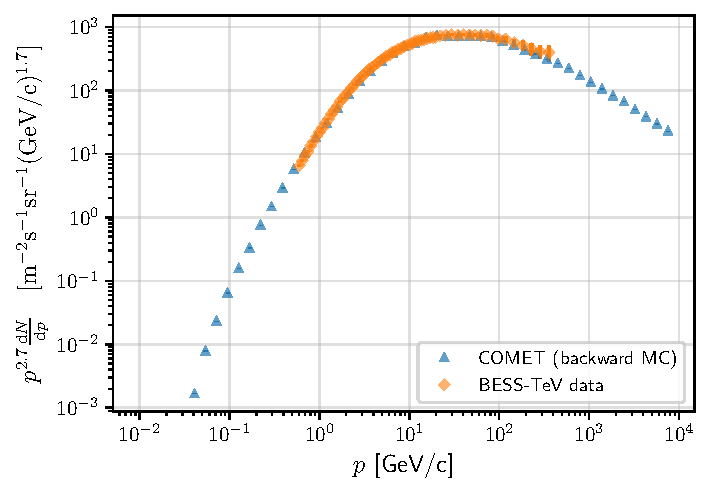
\includegraphics[width=0.95\textwidth]{chapter5/comparison_besstev.pdf}
        \caption{
            Comparison to data from the BESS-TeV spectrometer,
            which measured the flux of atmospheric muons at a vertical zenith
            angle in Manitoba, Canada~\cite{besstev}. }
    \end{subfigure}
    \hfill
    \begin{subfigure}[t]{0.49\textwidth}
        \centering
        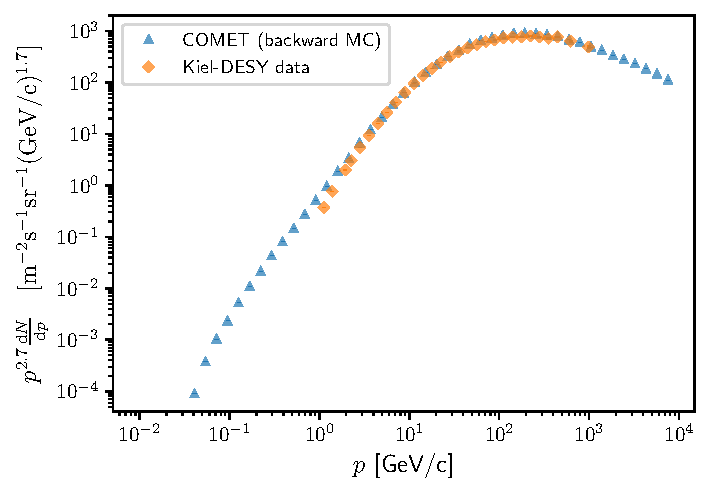
\includegraphics[width=0.95\textwidth]{chapter5/comparison_kieldesy.pdf}
        \caption{ 
            Comparison to the Kiel-DESY spectrometer observation of the
            atmospheric muon flux at a zenith angle of $\SI{75}{\degree} \pm
            \SI{7}{\degree}$~\cite{kieldesy} in Hamburg, Germany.}
    \end{subfigure}
    \caption{
        Validations of the backward MC results using experimental observations of the
        atmospheric muon flux by two independent experiments. Events from the
        backward MC simulation are selected to reflect the observational setup of
        the corresponding experiment, namely the respective incident angle at
        which muons were measured. Note that the backward MC data is obtained in
        a realistic simulation of the COMET experiment, taking into account the
        surrounding material and magnetic field, as well as the topography
        around of the J-PARC location.
    }
    \label{fig:bmc_validations}
\end{figure}

\begin{figure}
    \centering
    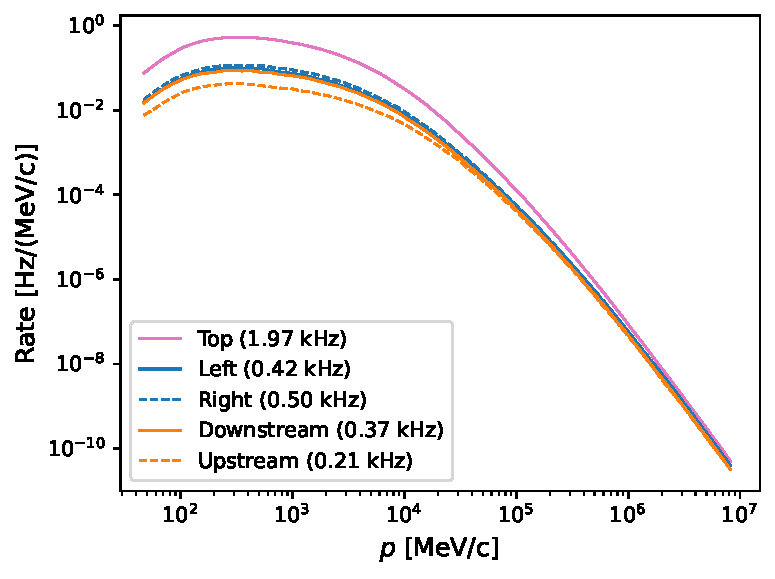
\includegraphics[width=0.5\textwidth]{chapter5/rate_vs_p.pdf}
    \caption{
        Average rate of inbound atmospheric muons over each face of the CRV as a
        function of momentum. Figures in parentheses in the legend are the
        integrated average rate over each face. In total, a rate of
        \SI{3.47}{\kHz} is expected.
    }
    \label{fig:avg_rate_per_face}
\end{figure}